\documentclass[12pt]{article}
%\renewcommand\normalsize{\fontsize{10pt}{12pt}\selectfont}
\usepackage{graphicx} % Required for inserting images
\usepackage[left=2cm,right=2cm,top=2cm,bottom=1.5cm]{geometry}

\title{PP}
%\author{Dennis Wilkinson}
\date{due Tuesday April 29}

\begin{document}

\setlength{\parindent}{0pt}
\setlength{\parskip}{3mm}

FS1 Wilkinson Practice problems from content in last two lectures

1. A long straight wire carrying a current $I$ creates a magnetic field of magnitude $B=\frac{\mu_0 I}{2\pi r}$ a distance $r$ from the wire. The unit will be Tesla (T) if you use SI units for the other quantities. As discussed in class, the direction of the field is circular around the wire. $\mu_0$ is a constant equal to $4\pi\times 10^{-7}$ T*m/A. 

\begin{figure}[h]
    \centering
    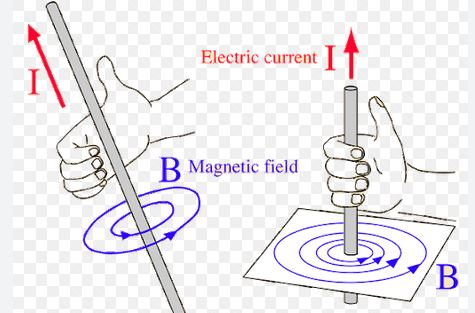
\includegraphics[width=0.5\linewidth]{wire B field.JPG}
\end{figure}

a. Find the strength of the field a distance 1 cm from a wire carrying current 1 A. 

b. Say the first wire carries current northward. A second wire is placed 1 cm to the east of this wire and also carries 1 A of current northward. The direction of the field from wire 1 at this location is downward, and the magnitude is what you found in part (a). Find the force, magnitude and direction, on one meter of the second wire. 

This force unit, $10^{-5}$ N, is also known as a dyne. According to some sources, but not others, the Ampere unit for current was defined as the current which would create 2 dynes of force per meter of wire. Other sources say it is 0.1A and 0.02 dynes. But why 2? Makes no sense to me. Maybe one dyne per wire or something? I don't have an answer.

c. What's one way to do this experiment on Earth, where the ambient field is $5\times 10^{-5}$ T, so the Earth's field (which is a lot stronger) doesn't corrupt the results?

d. What if one of the wires is carrying current in the opposite direction? What if they both are? 

\bigskip
\bigskip

2. a. Explain the difference between paramagnetic and ferromagnetic materials.

b. Explain how an electromagnet works.

\newpage

3. A simple schematic of a generator is pictured below.

\begin{figure}[h]
    \centering
    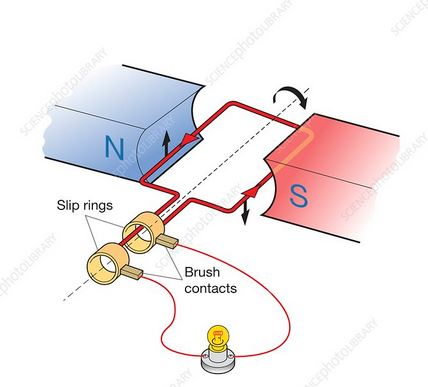
\includegraphics[width=0.4\linewidth]{generator.JPG}
\end{figure}

a. The B field lines point from N to S. Which way will the current run in the left side of this loop (near ``N") , at the moment pictured? It may or may not be in the direction of the red arrow.

b. Is the magnetic flux to the right (N to S) increasing or decreasing at this moment?

c. Which way is the magnetic \textit{force} (caused by the induced current) on the left side of the loop (near the ``N") at this moment? What about the right side? This is known as a counter torque.

d. Describe or draw the loop's orientation when the current is just about to reverse and flow the other way.

e. The slip rings here are \textbf{different from} the commutator in a DC motor. DC motor commutators make the current switch directions. These slip rings only keep the coil in contact with the wire. Will the current in the lightbulb be DC or AC? If DC, explain why. If AC, how does the light bulb stay on?

f. The voltage in the wire will equal $\omega NBA \sin \omega t$, where $\omega t$ is the angle between the coil (really, a vector perpendicular to the coil) and the field. The angle varies with time and the sine varies from $+1$ to $-1$; that's why the voltage is alternating. At the moment pictured in the drawing, the angle is 90 degrees. If we are turning the coil 2 times a second, there are $N=100$ loops in the coil, it's a square of side length 2 cm, what field do we need to generate 1 V of AC at this moment?

\bigskip
\bigskip

4.a.  Explain why it takes more energy to keep the coil rotating in a power plant when electricity demand increases. 

b. Explain what happens in a wind generation plant when energy demand is lower than energy supply.

\newpage

5. A DC motor has a coil which is attached to a battery as shown. 
\begin{figure}[h]
    \centering
    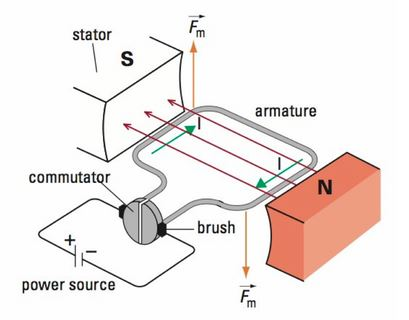
\includegraphics[width=0.5\linewidth]{motor.JPG}
\end{figure}

a. Explain why the commutator would not be necessary if the power source was AC instead of DC. What restriction does this put on the motor's spin rate? (To control the spin rate, we would need an electronic controller for the frequency - I believe they are called frequency drives. Perhaps gearing could also be used downstream from the motor.)

b. The coil is turning in the field, because it is attached to the power source. Thus, it is acting like a generator, and a current is induced. What direction is the magnetic force on electrons in the left side of the coil (near ``S") at the moment shown, when that side of the coil is moving upward? This is known as a \textbf{back EMF} or \textbf{back voltage}. It opposes the power source and lowers the current in the motor's windings.

c. Imagine that the motor is being used to power a pump, but the pump gets partially blocked, so the motor slows down and ``has to work harder". Explain what is happening, in terms of the back voltage and the power from the power source. 

d. If the motor is completely blocked, the back voltage drops to zero. What happens to the current in the coil? This is why motors can burn out.

\bigskip
\bigskip

6a. A transformer outside someone's house is taking 1440 V rms on the primary, which is a neighborhood supply line, down to 120 V rms in the secondary, which is the house line. If the primary has 200 turns in its coil, how many turns in the secondary?

b. Why don't transformers work with DC?

\newpage

Answers:

1a. $2\times 10^{-7}$ T. 

b. Force is west (the wires attract), magnitude is $2\times 10^{-5}$ N. 

c. I'm not sure what they did, but possibly they could run the wires north-south so the Earth's field exerts no force.

d. If one, the wires repel. If both, attract.

2a. You can look online, but one relatively concise answer is that unpaired electron spins in paramagnetic materials don't affect each other, so are mostly random from thermal jostling even within a strong external B field. In ferromagnetic materials, neighboring atoms align and can overcome the randomness. 

By the way, the presentation in class that Curie temperature defines the difference between soft and hard ferromagnets is an oversimplification, because there are various forms of randomness in material. 

And also by the way, a (simplified) reason that a compass needle pivots to align with the Earth's B, instead of the domains realigning, is that the needle is a relatively hard ferromagnet, so that it would take a very strong external field to realign the domains. The Earth's field is not that strong, so instead, the needle spins.

b. A piece of iron (or some ferromagnetic alloy) is placed within a solenoid, and current is run through the wire. This creates a B field in the iron, which is strongly increased when the domains align. 

\begin{figure}[h]
    \centering
    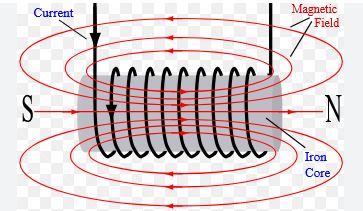
\includegraphics[width=0.5\linewidth]{electromagnet.JPG}
\end{figure}

3a. Into the paper, away from the rings (v is up, B to right)

b. Increasing

c. down on left, up on right - this is counter torque, the motor effect

d. Vertical, turned 90 degrees from how it is in the picture

e. AC. The lightbulb filament will be heated by the AC, because resistance heating happens even if the current is switching. The filament will stay hot and glow.

f. 1.98 T. Very large! We probably need a bigger coil, or a higher spin rate. Remember that $\omega=2\pi$ times the number of rotations per second. 

4a. Because there is more current in the coil, creating more counter torque.

b. The counter torque is too low for safe operating speed if too many turbines are allowed to turn, so they have to shut down some of the towers (I believe there is a remote-controlled brake which stops the blades from spinning).

5a. AC switches direction anyway, so the motor would turn. However, it could turn only at the frequency of the AC.

b. the force on the electrons is into the paper (away from the commutator), but electrons move in the opposite direction from $I$, so the motion induces a voltage/current that opposes $I$/the power source - the back voltage.

c. The spin rate is slower, so there is less back voltage. Thus the current in the wire \textit{increases} (counterintuitively) and the power source is doing more work.

d. The current could get so high that the wires heat up and potentially fail. 

6a. 20

b. Because the B field in the iron core is not changing, so there is no induced voltage in the secondary.

\end{document}